\documentclass[11pt]{article}

\pdfobjcompresslevel=3    % compress PDF objects
\pdfcompresslevel=9       % compress streams more (0..9)
\pdfminorversion=4


\usepackage[utf8]{inputenc} % remove if using XeLaTeX or LuaLaTeX
\usepackage[T1]{fontenc}
\usepackage{polski}[babel]

% Layout & graphics
\usepackage[a4paper, total={7.5in, 9in}]{geometry}
\usepackage{graphicx}
\usepackage{wrapfig}              % images
\usepackage[dvipsnames,table]{xcolor} % single xcolor invocation (keeps table option)

% Math & symbols
\usepackage{amsmath}
\usepackage{amssymb}
\usepackage{gensymb}

% Typography & layout helpers
\usepackage{microtype}
\usepackage{float}                 % [H] placement
\usepackage{caption}
\usepackage{subcaption}            % modern subfigure support (do NOT load subfig)
\usepackage{multirow}
\usepackage{titlesec}

\usepackage{lmodern}
\usepackage{microtype}
\usepackage{listings}
\usepackage{xcolor}

\lstdefinestyle{MyStyle}{
    basicstyle=\ttfamily\small, % Font family and size
    keywordstyle=\color{blue}\bfseries, % Style for keywords
    commentstyle=\color{green!60!black}\itshape, % Style for comments
    %stringstyle=\color{red}, % Style for strings
    numberstyle=\tiny\color{gray}, % Style for line numbers
    backgroundcolor=\color{gray!10}, % Background color
    frame=single, % Add a frame around the code block
    breaklines=true, % Allows long lines to wrap
    language=Java, % Default language
    numbers=left, % Line numbers on the left
    showstringspaces=false % Don't show spaces in strings
}

\lstset{style=MyStyle}

\definecolor{xppblue}{RGB}{37, 150, 190}

\title{Sprawozdanie 2 z laboratorium \par Układy sterowania optymalnego}
\author{Jan Andrzejewski 159512}
\date{}

\begin{document}

\maketitle

\tableofcontents

\newpage

\section{Ćwiczenie 10-11: Linearyzacja systemu nieliniowego}


\begin{figure}[H]
    \centering
    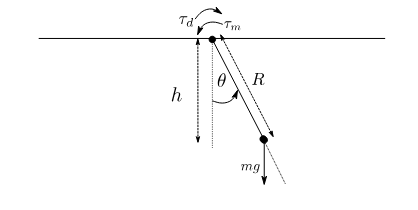
\includegraphics[width=0.6\linewidth]{img/wahadlo.png}
    \caption{Schemat napedzanego wahadła}
\end{figure}

Rozważany jest model napędzanego wahadła będący obiektem nieliniowym. Przyjmując $x_1=\theta$ (położenie kątowe) i $x_2=\dot{\theta}$ (prędkość kątowa), równania stanu systemu przyjmują postać:

\[
\dot{x}_1=x_2
\]
\[
\dot{x}_2=\frac{1}{J}u-\frac{d}{J}x_2-\frac{mgl}{J}\sin(x_1)
\]

gdzie $J=1$ kg·m², $d = 0.5$ N·m·s/rad, $m = 9$ kg, $l = 1$ m.

\subsection{Linearyzacja wokół punktu $x_0=[0,0]$, $u=0$}

Przeprowadzono linearyzację układu wokół punktu pracy $(x_0=[0,0], u_0=0)$. Dla tego punktu pracy macierze liniowego modelu przyjmują postać:

\[
A = \begin{bmatrix}
    0 & 1\\
    -\frac{mgl}{J} & -\frac{d}{J}
\end{bmatrix}, \quad
B = \begin{bmatrix}
    0\\
    \frac{1}{J}
\end{bmatrix}
\]

Podstawiając parametry:

\[
A = \begin{bmatrix}
    0 & 1\\
    -90 & -0.5
\end{bmatrix}, \quad
B = \begin{bmatrix}
    0\\
    1
\end{bmatrix}
\]

Układ jest sterowalny, ponieważ rząd macierzy Kalmana jest równy wymiarowi systemu:
\[
\text{rank}([B, AB]) = 2
\]

Rank macierzy $A$ wynosi 2, a rank macierzy sterowalności również wynosi 2. Dodatkowo, forma zaobserwowana macierzy $A$ jest formą kanoniczną, co wskazuje na pełną sterowalność systemu.

\textbf{Porównanie odpowiedzi nieliniowej i liniowej:}

\begin{figure}[H]
    \centering
    \includegraphics[width=0.7\linewidth]{img/lininielin5.png}
\end{figure}

\begin{figure}[H]
    \centering
    \includegraphics[width=0.7\linewidth]{img/lininielin45sqrt.png}
\end{figure}

Z przebiegów można wyciągnąć jednoznaczny wniosek: linearyzacja wokół punktu pracy dobrze opisuje model tylko w jego bezpośrednim otoczeniu. Dla małych zaburzeń od punktu równowagi przebieg zmiennej z modelu zlinearyzowanego pokrywa się z przebiegiem modelu nieliniowego. Jednak przy zwiększaniu odchylenia od punktu pracy dokładność linearyzacji spada. Daje się zaobserwować wyraźne odchylenia między modelem liniowym i nieliniowym dla wejścia $45\sqrt{2}$.

\subsection{Linearyzacja wokół punktu $x_0=[\pi/4,0]$, $u=45\sqrt{2}$}

Dla drugiego punktu pracy macierze liniowego modelu przyjmują postać:

\[
A = \begin{bmatrix}
    0 & 1\\
    -\frac{mgl}{J}\cos(\pi/4) & -\frac{d}{J}
\end{bmatrix}, \quad
B = \begin{bmatrix}
    0\\
    \frac{1}{J}
\end{bmatrix}
\]

Podstawiając parametry:
\[
A = \begin{bmatrix}
    0 & 1\\
    -63.64 & -0.5
\end{bmatrix}
\]

W przypadku linearyzacji wokół punktu innego niż $x_0=\begin{bmatrix} 0 & 0 \end{bmatrix}$, należy wprowadzić nowe zmienne $\tilde{x}=x-x_0$ i $\tilde{u}=u-u_0$. Ostatecznie otrzymano równania stanu w postaci:
\[
\dot{\tilde{x}}=A\tilde{x}+B\tilde{u}
\]

Nowy zlinearyzowany system interpretuje punkt, wokół którego został zlinearyzowany, jako swój nowy punkt równowagi. Dlatego to przesunięcie musi być wzięte pod uwagę.

Przebieg położenia przy wytraceniu układu z równowagi warunkami początkowymi $x_0=\begin{bmatrix}
    \pi/4 & 0
\end{bmatrix}$:


\begin{figure}[H]
    \centering
    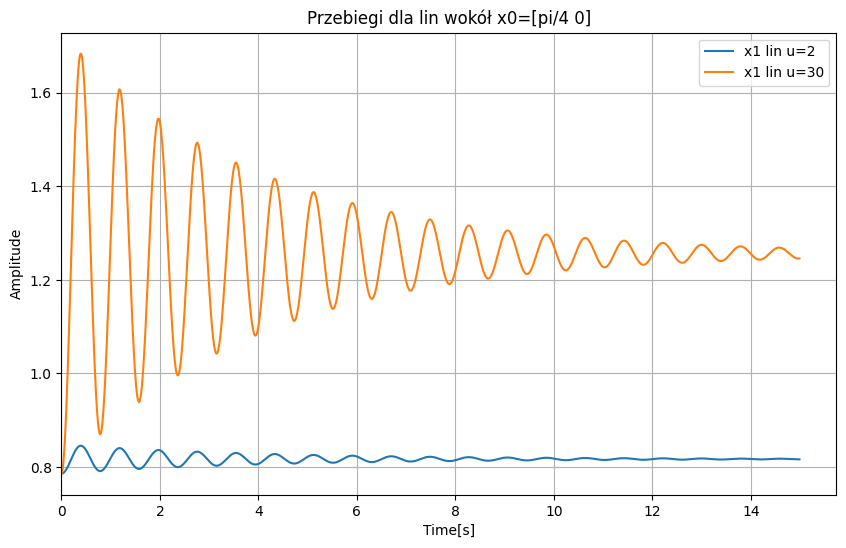
\includegraphics[width=0.7\linewidth]{img/linpi4.png}
    \caption{Porównanie przebiegów modelu nieliniowego i zlinearyzowanego dla wymuszeń stałych}
\end{figure}

Analogicznie do zadania 1.1, model zlinearyzowany prawidłowo opisuje zachowanie systemu w otoczeniu punktu pracy. Odchylenia rosną wraz ze wzrostem odległości od punktu równowagi.

\subsection{Linearyzacja metodą SDC}

Metoda SDC polega na dyskretyzacji systemu w każdym kroku czasowym wokół bieżącego stanu, a następnie rozwiązaniu równań dyskretnych. Parametry macierzy $A$ są aktualizowane w zależności od bieżącego stanu systemu:

\[
\dot{x}=\begin{bmatrix}
    0 & 1 \\
    -\frac{mgl}{J}\frac{\sin(x_1)}{x_1} & -\frac{d}{J} 
\end{bmatrix}x+\begin{bmatrix}
    0 \\ \frac{1}{J}
\end{bmatrix}u
\]

dla $x_1 \neq 0$, co pozwala na lepsze śledzenie nieliniowych zmian systemu w porównaniu ze statyczną linearyzacją.

\begin{figure}[H]
    \centering
    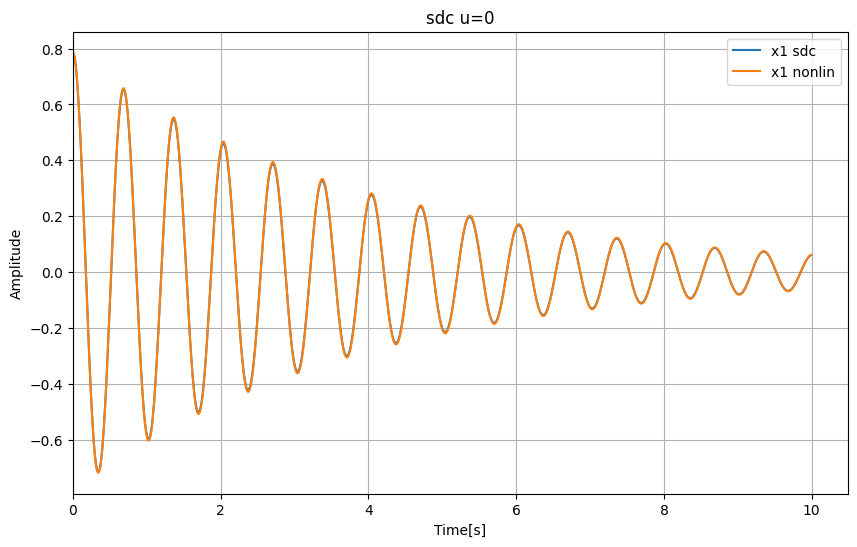
\includegraphics[width=0.7\linewidth]{img/sdcu0.png}
\end{figure}

\begin{figure}[H]
    \centering
    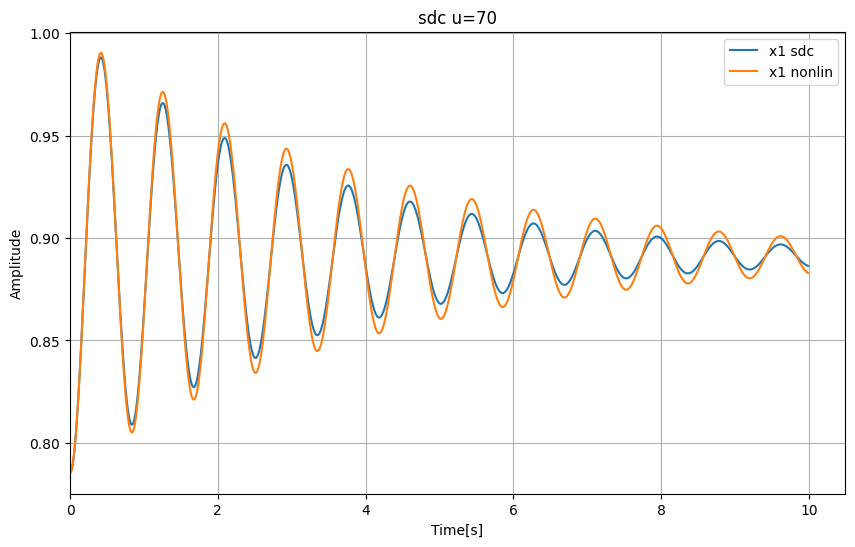
\includegraphics[width=0.7\linewidth]{img/sdcu70.png}
\end{figure}



Metoda SDC oferuje lepszą dokładność niż klasyczna linearyzacja, ponieważ parametry modelu są adaptacyjnie aktualizowane na podstawie bieżącego stanu. Pozwala to na śledzenie trajektorii daleko od punktu linearyzacji. Pomimo zalet metody SDC można zaobserwować rozbieżności dla dużych wielkości wejść. Dla dużych oscylacji rozbieżność między $\frac{\sin(x_1)}{x_1}$ a $\sin(x_1)$ rośnie.

\newpage

\subsection{Kod wyznaczający odpowiedź z użyciem parametryzacji SDC}

\begin{lstlisting}
    m, l, J, g, d = 9.0, 1.0, 1.0, 10.0, 0.5
t_sim = np.arange(0, 10, 0.01)

x_0 = [np.pi/4, 0] # x1 = theta, x2 = theta_dot
results_sdc = [x_0]

curr_x = x_0

for i in range(len(t_sim) - 1):
    x1, x2 = curr_x
    
    if abs(x1) < 1e-6:
        a21 = -(m * g * l) / J
    else:
        a21 = -(m * g * l / J) * (np.sin(x1) / x1)
    
    A = [[0, 1],
         [a21, -d/J]]
    B = [[0], [1/J]]
    C = [[1, 0], [0, 1]]
    D = [[0], [0]]
    
    sys = signal.StateSpace(A, B, C, D)
    
    t_step = [0, 0.01]
    u_step = [0, 0] 
    
    _, _, x_out = signal.lsim(sys, U=u_step, T=t_step, X0=curr_x)
    
    curr_x = x_out[-1]
    results_sdc.append(curr_x)

results_sdc = np.array(results_sdc)
    
\end{lstlisting}


\section{Ćwiczenie 12: Regulator LQR dla układów nieliniowych}

\subsection{Linearyzacja modelu wahadła wokół punktu $x_0 = [\pi, 0]$, $u_0 = 0$ }

Rozpatrywany jest napędzany model wahadła analogiczny do ćwiczenia 10-11:

\[
\dot{x}=\begin{bmatrix}
    0 & 1 \\
    -\frac{mgl}{J}\sin(x_1) & -\frac{d}{J}
\end{bmatrix}x + \begin{bmatrix}
    0 \\ \frac{1}{J}
\end{bmatrix}u
\]

Linearyzacja wokół punktu $x_0 = [\pi, 0]$, $u_0 = 0$ daje:

\[
A = \begin{bmatrix}
    0 & 1\\
    -\frac{mgl}{J}\cos(\pi) & -\frac{d}{J}
\end{bmatrix} = \begin{bmatrix}
    0 & 1\\
    \frac{mgl}{J} & -\frac{d}{J}
\end{bmatrix}
\]

\[
B = \begin{bmatrix}
    0\\
    \frac{1}{J}
\end{bmatrix}
\]

Z podstawionymi wartościami ($m=9$, $g=9.81$, $l=1$, $J=1$, $d=0.5$):

\[
A = \begin{bmatrix}
    0 & 1\\
    88.29 & -0.5
\end{bmatrix}, \quad
B = \begin{bmatrix}
    0\\
    1
\end{bmatrix}
\]

Punkt równowagi $x_0 = [\pi, 0]$ odpowiada wahadłu w pozycji pionowej. Jest to równowaga niestabilna:

\begin{lstlisting}
    np.linalg.eigvals(A) #array([ 9.14960106, -9.64960106])
\end{lstlisting}

Wartości własne macierzy $A$ odpowiadające biegunom systemu wskazują na jego niestabilność: jeden biegun stabilny i jeden biegun niestabilny.

\subsection{Projektowanie regulatora LQR}

Zaprojektowano regulator LQR minimalizujący wskaźnik jakości:
\[
J = \int_0^\infty (x^T Q x + u^T R u) dt
\]

Z macierzami wag:
\[
Q = I_2 = \begin{bmatrix} 1 & 0 \\ 0 & 1 \end{bmatrix}, \quad R = 1
\]

Rozwiązując ARE otrzymano wzmocnienia regulatora:

\[
K=\begin{bmatrix}
    176,5 & 18,3
\end{bmatrix}
\]

Prawo sterowania uwzględniające punkt, wokół którego układ został zlinearyzowany:
\[
\tilde{u} = -K(x - x_0) + u_0
\]


\begin{figure}[H]
    \centering
    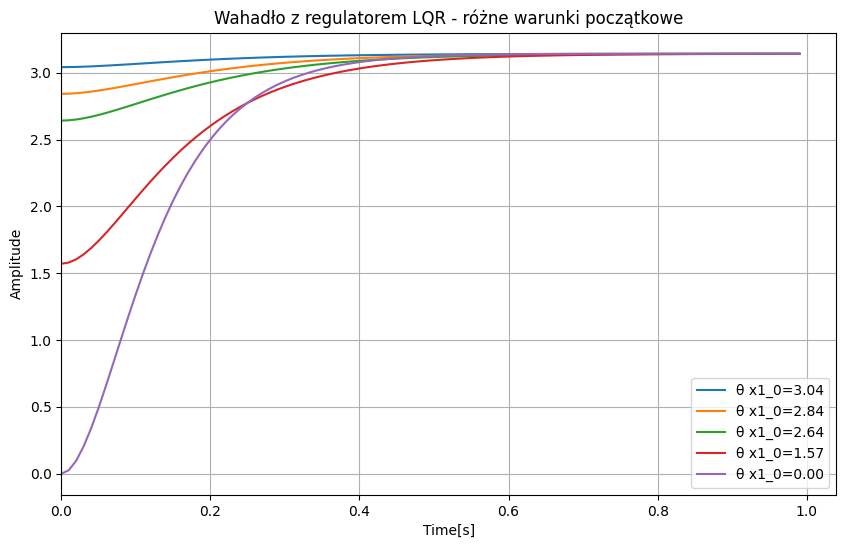
\includegraphics[width=0.8\linewidth]{img/lqrpoczatkowe.png}
\end{figure}

Otrzymane rozwiązanie nie jest globalne. Regulator LQR jest projektowany dla liniowego modelu systemu wokół punktu równowagi $[\pi, 0]$. Jego działanie jest gwarantowane jedynie dla małych zaburzeń wokół tego punktu. Dla większych odchyleń (np. wahadło bliskie pozycji dolnej $[0, 0]$) liniowy model nie reprezentuje już dokładnie dynamiki systemu nieliniowego, a regulator traci swoją efektywność. Biorąc to pod uwagę można wyciągnąć wniosek, że przebiegi dla dużych odchyleń nie mają jakiegokolwiek pokrycia z tym co można by zaobserwować w rzeczywistości. Implementując regulator przy założeniu takiej linearyzacji i nie startując z otoczenia warunków początkowych $x_0=\begin{bmatrix}
    \pi & 0
\end{bmatrix}$, nie zostałby odwzorowany taki przebieg jak w symulacji. 

\subsection{Manipulator elastyczny}

\begin{figure}[H]
    \centering
    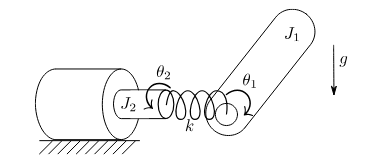
\includegraphics[width=0.6\linewidth]{img/manipulator.png}
\end{figure}

Rozpatrywany jest manipulator z elastycznym złączem opisany równaniami:
\[
J_1\ddot{\theta}_1 + mgl\sin(\theta_1) + k(\theta_1 - \theta_2) = 0
\]
\[
J_2\ddot{\theta}_2 - k(\theta_1 - \theta_2) = u
\]

gdzie $J_1 = 0.04$ kg·m², $J_2 = 0.3$ kg·m², $k = 3$ N/m, $m = 0.5$ kg, $l = 0.5$ m.

Ze zmiennymi stanu $x = [\theta_1, \dot{\theta}_1, \theta_2, \dot{\theta}_2]^T$ równania stanu przyjmują postać:
\[
\dot{x}_1 = x_2
\]
\[
\dot{x}_2 = \frac{1}{J_1}(-mgl\sin(x_1) - k(x_1 - x_3))
\]
\[
\dot{x}_3 = x_4
\]
\[
\dot{x}_4 = \frac{1}{J_2}(u + k(x_1 - x_3))
\]

W postaci macierzowej:
\[
\dot{x} = \begin{bmatrix}
    0 & 1 & 0 & 0 \\
    -\frac{mgl}{J_1}\sin(x_1) - \frac{k}{J_1} & 0 & \frac{k}{J_1} & 0 \\
    0 & 0 & 0 & 1 \\
    \frac{k}{J_2} & 0 & -\frac{k}{J_2} & 0
\end{bmatrix} x + \begin{bmatrix}
    0 \\ 0 \\ 0 \\ \frac{1}{J_2}
\end{bmatrix} u
\]

\subsection{Linearyzacja wokół punktu $x_0=\begin{bmatrix}0&0&0&0\end{bmatrix}$ i $u_0=0$}

\[
A = \begin{bmatrix}
    0 & 1 & 0 & 0 \\
    -\frac{mgl + k}{J_1} & 0 & \frac{k}{J_1} & 0 \\
    0 & 0 & 0 & 1 \\
    \frac{k}{J_2} & 0 & -\frac{k}{J_2} & 0
\end{bmatrix}, \quad
B = \begin{bmatrix}
    0 \\ 0 \\ 0 \\ \frac{1}{J_2}
\end{bmatrix}
\]

Podstawiając wartości parametrów:

\[
A = \begin{bmatrix}
    0 & 1 & 0 & 0 \\
    -137.5 & 0 & 75 & 0 \\
    0 & 0 & 0 & 1 \\
    10 & 0 & -10 & 0
\end{bmatrix}, \quad
B = \begin{bmatrix}
    0 \\ 0 \\ 0 \\ 3.33
\end{bmatrix}
\]


\subsection{Wpływ S, Q i R na przebiegi}

\begin{figure}[H]
    \centering
    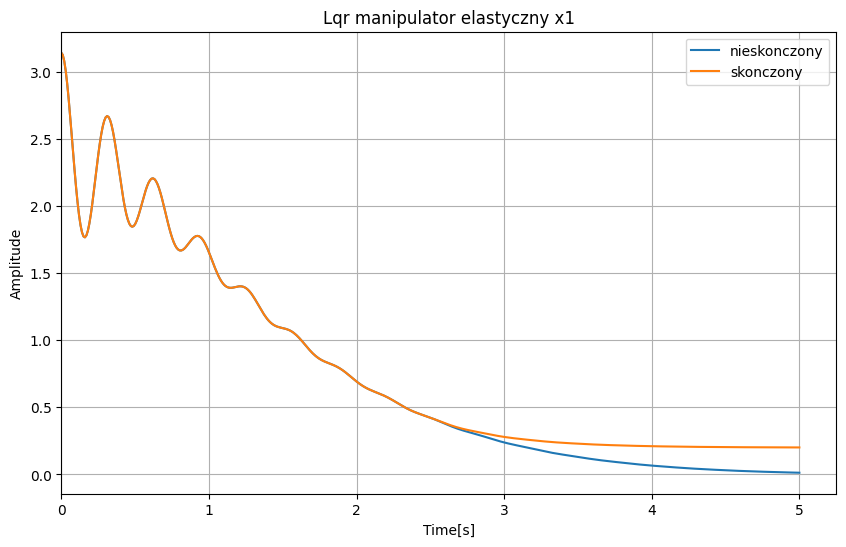
\includegraphics[width=0.8\linewidth]{img/lqrmanipulatorpolozenie.png}
    \caption{Symulacja dla $S=I_4$}
\end{figure}
 

\begin{figure}[H]
    \centering
    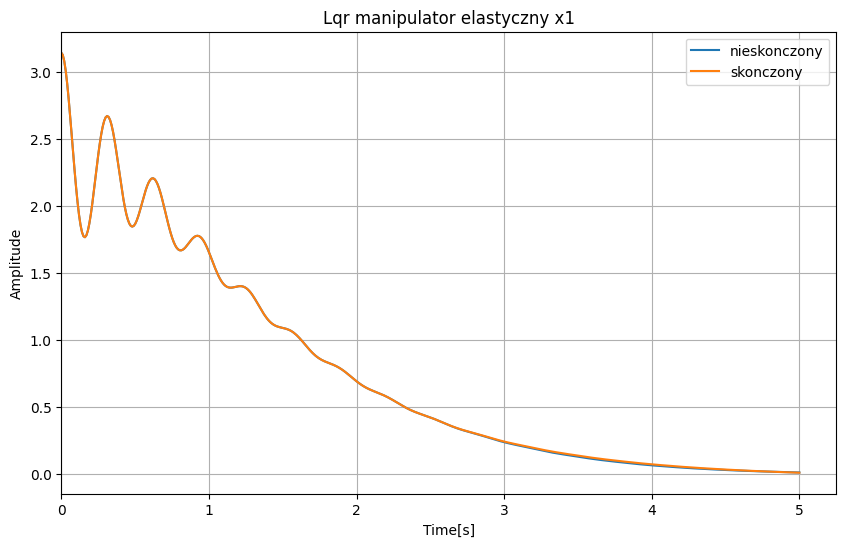
\includegraphics[width=0.8\linewidth]{img/lqrmanipulatorS.png}
    \caption{Symulacja dla $S=I_4 \cdot 0.5$}
\end{figure}

Wyraźnie widac ze macierz S zgodnie z

TODO dalej 3.4




\end{document}